%%%%%%%%%%%%%%%%%%%%%%%%%%%%%%%%%%%%%%%%%
% Beamer Presentation
% LaTeX Template
% Version 1.0 (10/11/12)
%
% This template has been downloaded from:
% http://www.LaTeXTemplates.com
%
% License:
% CC BY-NC-SA 3.0 (http://creativecommons.org/licenses/by-nc-sa/3.0/)
%
%%%%%%%%%%%%%%%%%%%%%%%%%%%%%%%%%%%%%%%%%

%----------------------------------------------------------------------------------------
%	PACKAGES AND THEMES
%----------------------------------------------------------------------------------------

\documentclass{beamer}

\mode<presentation> {

% The Beamer class comes with a number of default slide themes
% which change the colors and layouts of slides. Below this is a list
% of all the themes, uncomment each in turn to see what they look like.

%\usetheme{default}
%\usetheme{AnnArbor}
%\usetheme{Antibes}
%\usetheme{Bergen}
%\usetheme{Berkeley}
%\usetheme{Berlin}
%\usetheme{Boadilla}
%\usetheme{CambridgeUS}
%\usetheme{Copenhagen}
%\usetheme{Darmstadt}
%\usetheme{Dresden}
%\usetheme{Frankfurt}
%\usetheme{Goettingen}
%\usetheme{Hannover}
%\usetheme{Ilmenau}
%\usetheme{JuanLesPins}
%\usetheme{Luebeck}
\usetheme{Madrid}
%\usetheme{Malmoe}
%\usetheme{Marburg}
%\usetheme{Montpellier}
%\usetheme{PaloAlto}
%\usetheme{Pittsburgh}
%\usetheme{Rochester}
%\usetheme{Singapore}
%\usetheme{Szeged}
%\usetheme{Warsaw}

% As well as themes, the Beamer class has a number of color themes
% for any slide theme. Uncomment each of these in turn to see how it
% changes the colors of your current slide theme.

%\usecolortheme{albatross}
%\usecolortheme{beaver}
%\usecolortheme{beetle}
%\usecolortheme{crane}
%\usecolortheme{dolphin}
%\usecolortheme{dove}
%\usecolortheme{fly}
%\usecolortheme{lily}
%\usecolortheme{orchid}
%\usecolortheme{rose}
%\usecolortheme{seagull}
%\usecolortheme{seahorse}
%\usecolortheme{whale}
%\usecolortheme{wolverine}

%\setbeamertemplate{footline} % To remove the footer line in all slides uncomment this line
%\setbeamertemplate{footline}[page number] % To replace the footer line in all slides with a simple slide count uncomment this line

%\setbeamertemplate{navigation symbols}{} % To remove the navigation symbols from the bottom of all slides uncomment this line
}

\usepackage{graphicx} % Allows including images
\usepackage{booktabs} % Allows the use of \toprule, \midrule and \bottomrule in tables
\usepackage{algorithm}
\usepackage{float}
\usepackage{algpseudocode}
%----------------------------------------------------------------------------------------
%	TITLE PAGE
%----------------------------------------------------------------------------------------

\title[Multiagent Systems course project]{Application of Deep Q-Learning techniques on a GridWorld environment} % The short title appears at the bottom of every slide, the full title is only on the title page

\author{Federico Vaccaro} % Your name
\institute[UniFi] % Your institution as it will appear on the bottom of every slide, may be shorthand to save space
{
Università degli studi di Firenze \\ % Your institution for the title page
\medskip
\textit{federico.vaccaro@stud.unifi.it} % Your email address
}
\date{October 9, 2020} % Date, can be changed to a custom date

\begin{document}

\begin{frame}
\titlepage % Print the title page as the first slide
\end{frame}

\begin{frame}
\frametitle{Overview} % Table of contents slide, comment this block out to remove it
\tableofcontents % Throughout your presentation, if you choose to use \section{} and \subsection{} commands, these will automatically be printed on this slide as an overview of your presentation
\end{frame}

%----------------------------------------------------------------------------------------
%	PRESENTATION SLIDES
%----------------------------------------------------------------------------------------

%------------------------------------------------
\section{Introduction} % Sections can be created in order to organize your presentation into discrete blocks, all sections and subsections are automatically printed in the table of contents as an overview of the talk
%------------------------------------------------
\subsection{Introduction to RL}
\begin{frame}
\frametitle{Paradigms of Machine Learning}
\begin{itemize}
	\item \textbf{Unsupervised learning}: learning without annotations;\\ 
	\textit{e.g.} K-means, Mean Shift, GMM...
	\item \textbf{Supervised learning}: learning with annotations:
	\\ \textit{e.g.} classification, regression with SVM, Decision Trees, Neural Networks...
	\item \textbf{Reinforcement learning}: learning \textit{policies for maximizing rewards}:\\
	\begin{itemize}
		\item Q-Learning
		\item Value iteration 
		\item Policy iteration
	\end{itemize}
\end{itemize}
\end{frame}

\begin{frame}
\frametitle{Reinforcement Learning}
	An environment $\mathcal{E}$ and the interaction with an agent modeled as a dynamical system: $s_{t+1} = f(s_t, a_t, \xi_t )$.\\ The purpose of the agent is to \textbf{maximize} the expected reward.
	
	\begin{equation}
\mathcal{V} = \mathbb{E}_\xi \{ (\sum_{t=0}^{T-1} r(t, s_t, a_t)) + r(s_T,t) \} % = \mathbb{E}_\xi \{ \sum_{t=0}^{\infty}R_t \} %
	\end{equation}
	
\begin{figure}[H]
	\centering
	\includegraphics[width=0.4\textwidth]{reinforcement}
	\label{fig:rl}
\end{figure}


\end{frame}

\begin{frame}
\frametitle{Reinforcement Learning}
Each of the three strategies is designed to obey a fundamental equation, in reinforcement learning, which is the \textbf{Bellman equation of the dynamic programming}.
\begin{theorem}[Bellman equation of the dynamic programming at infinite horizon] 
	$
	R_t =  \alpha^t r(s_t, a_t)$ 
	\\
	$\mathcal{V} = \sum_{t=0}^{\infty}R_t \text{ is limited if $r$ is limited}
	$
	\\
	$ \alpha \in (0,1) $
	\\
	\begin{equation}
	\begin{aligned}
	\mathcal{V}^o(s_t,t) = \max_{a_t}
	\bigg\{ r(s_t, a_t) + \alpha\mathcal{V}^o(s_{t+1}, t+1) \bigg\} \\
	\gamma^o(s_t, t) = \arg \max_{a_t} 		\big\{ \mathcal{V}^o(s_t,t)\big\}
	\end{aligned}
	\end{equation}

\end{theorem}

\end{frame}
%------------------------------------------------
\begin{frame}
\subsection{Q-Learning}
\frametitle{Q-Learning}
We can define the \textbf{action-value function} $Q(s,a) $. The $Q$ function is the result of \textbf{applying} the action $a$ while in the state $s$, getting the reward, and adding the discounted \textbf{expected reward} from the next state $s_{t+1}$ obtained by applying the optimal policy $\gamma^o(s_{t+1}, t+1)$.
\begin{equation}
	Q(s_t,a_t) = r(s_t, a_t) + \alpha \mathcal{V}^o(s_{t+1}, t+1)
\end{equation}
\begin{theorem}[$Q^\star$ satisfies the Bellman equation]
	$Q^\star(s_t, a_t) = \max_{a} Q(s_t, a)$ \\
	$\mathcal{V}^o(s_t, t) = Q^\star(s_t, a_t)$ by definition \\
	$ \implies	Q^\star (s_t,a_t) = r(s_t, a_t) + \alpha \max_{a'} Q(s_{t+1}, a_{t+1})$
\end{theorem}
Therefore, the optimal policy $\gamma^o(s_0, 0)$ is simply defined by \textbf{selecting at each time-step} the action with \textbf{higher Q-score}. \\
Issue: \textbf{curse of dimensionality}! Complex to solve when state space $\mathbb{X}$ or action space $\mathbb{U}$ are large!
\end{frame}

\section{Deep Q-Learning}
\begin{frame}
	\frametitle{Approximating the Q-function}
	To counter the course of dimensionality, we can think to \textbf{approximate} the Q-function with a Neural Network, which is a \textbf{universal function approximator}, parametrized with a set of weights and biases $\theta$.
	\begin{equation}
		Q(s, a) \approx Q(s,a| \theta)
	\end{equation}
	It is trained with a \textbf{regression} over the Bellman equation.
		\begin{equation}
\begin{aligned}
y_i =  r + \alpha \max_{a'} Q(s', a'|\theta_{i-1}) \\
L_i(\theta _i ) = (y_i - Q(s,a|\theta_i))^2
\end{aligned}
	\end{equation}
Note that this method is \textbf{model-free}, \textit{i.e.} it has no prior knowledge/estimation of the environment $\mathcal{E}$, but it directly observe its "external" state.
\end{frame}
\subsection{Deep Q-Learning tricks}

\begin{frame}
\frametitle{Replay Memory}

At each time-step, we collect a tuple from the experience of the agent: $e_t = (s_t, a_t, s_{t+1}, r_t)$. We mantain these experiences in a pool, which we refer as \textbf{replay memory}. Then, we are abilitated to sample mini-batches of tuples from this data-structure.

This is efficient for two reasons: 
\begin{enumerate}
	\item it allows to build minibatches of \textbf{indipendent samples}, which are mandatory for a correct estimation of the gradient via SGD;
	\item it is \textbf{computationally-efficient}, since we can leverage parallel-computing hardware and optimized software.
\end{enumerate}

\end{frame}

\begin{frame}
\frametitle{\textit{Exploration-exploitation} trade-off}
 During the first stages of training, the parameters are close to being randomly initialized, then the output Q-scores have really few sense, then choosing the \textit{greedy} action hardly is the best option. Before achieving a meaningful approximation, with a probability of $\epsilon$ we select a random action ($1 - \epsilon$ selects the greedy action) during the training. As the agent keep accumulating experience and training, $\epsilon$ will tend to decrease, letting the agent improving the learned policies. We refer to this mechanism as \textbf{exploration-exploitation} trade-off: in my\label{our} experiments, the value is initialized at $0.9$, and linearly decays to $0.1$ at the $25\%$ of completion of the training.\\~\\
 This technique makes the Deep Q-Learning \textbf{off-policy}, because it does not learn by directly sampling from a policy (a sequence of steps), but rather training on different actions, even randomly sampled.
\end{frame}

\subsection{DQL training algorithm}
\begin{frame}{DQL training algorithm}
	\begin{center}
	\scalebox{0.7}{
		    \begin{minipage}{1.1\linewidth}
			
\begin{algorithm}[H]
	\caption{Deep Q-Learning algorithm}
	\begin{algorithmic}
		\State Initialize ReplayMemory $\mathcal{D}$ with capacity N
		\State Initialize DQN $Q(x, a|\theta)$ with random weights $\theta_0$
		\For{episode $1,M$}
		\State Initialize sequence $s_0=\{x_1\}$
		\For{$t=1,T$}
		\State With probability $\epsilon_{ep}$ select the random action $a_t$ 
		\State otherwise select $a_t=\max_{a}Q(x_t, a|\theta)$
		\State Execute $a_t$ and observe reward $r_t$ and state change $x_{t+1}$
		\State set sequence $s_{t+1}=(x_t, a_t, x_{t+1}, r_t)$ 
		\State store sequence $s_{t+1}$ in $\mathcal{D}$
		\State sample a minibatch of $B$ transitions $s_j=(x_j, a_j, x_{j+1}, r_j)$
		\State set $y_j = 
		\begin{cases}
		r_t \text{ if $x_{t}$ is terminal} \\
		r_t + \gamma\max_{a'}Q(x_{t+1}, a'|\theta) \text{ otherwise}
		\end{cases}
		$
		\State Compute $L(\theta) = \sum_{j}^{B} \frac{1}{B} (y_j - Q(x_j, a_j|\theta) )^2 $
		\State Perform a gradient descent update based on $\nabla_\theta L\theta$
		\EndFor		
		\EndFor
	\end{algorithmic}
\end{algorithm}
\end{minipage}
}
	\end{center}
\end{frame}

\subsection{Double Deep Q-Learning}
\begin{frame}{Double Deep Q-Learning}
	\begin{itemize}
	\item Sometimes the model learn unrealistically high action values because it includes a maximization step over estimated action values, which tends to prefer overestimated to underestimated values. 
	\item We can decopule the \textbf{training network} from the \textbf{target values network} $y_i$ (\textit{i.e.} into two network with parameters $\theta$ and $\theta^t $). If we expand the equation, then we obtain (in a deterministic environment):
	\end{itemize}

	\begin{equation}
	\label{doubleql}
	\begin{aligned}
	y_i =  r + \alpha \max_{a'} Q(s', a'|\theta) = \\
	r + \alpha Q(s', \arg \max_a Q(s', a|\theta)  |\theta)
	\end{aligned}
	\end{equation}
	The Eq. \ref{doubleql} becomes
	\begin{equation}
	r + \alpha Q(s', \arg \max_a Q(s, a|\theta)  |\theta^t)
	\end{equation}
	During the training, the roles of the two Q-network will be switched after a number of steps. 
\end{frame}

\section{The experiment}
\subsection{Environment definition}
\begin{frame}{The \textit{GridWorld} game}
	\begin{columns}[c] % The "c" option specifies centered vertical alignment while the "t" option is used for top vertical alignment
		
		\column{.45\textwidth} % Left column and width
\begin{figure}
	\centering
	\includegraphics[width=1.2\textwidth]{game_example}
	\label{fig:game1}
\end{figure}
		
		\column{.6\textwidth} % Right column and width
	\begin{itemize}
	\item The state is a tensor of dimension $16 \times 16 \times 3$;
	\item The agent can move the green square at each step the green square in one of the four direction (up, right, down, left);
	\item The goal is to avoid the obstacles (black cells) and reach the arrival point (red square).
	\item There are $16\times16$ reachable position for the agent, multiplied by all the possible start and finish combinations which are more than $\sim 60$. The number of possible states then is over $15360$.
\end{itemize}
		
	\end{columns}
	
	


\end{frame}

\begin{frame}{Environment reward system}
	The reward system works as follows:
	\begin{itemize}
		\item $r_t = 1$ If the agent gets the green closer to the ending square but in a white cell;
		\item $r_t = -1$ If the agent moves the green square upon an obstacle;
		\item $r_t = -1$ If the agent enters again in a cell already visited (for discouraging loops) \textbf{or} tries a move towards a wall;
		\item $r_t = 2$ If the agent can reach the red square;
		\item $r_t = 0$ If the agent gets farther from the objective, but in a white cell not visited yet.
	\end{itemize}
	The game terminates when the agent reach the green square; otherwise we adopted an early exit strategy, meaning when the game cumulative reward reaches a negative score of $-500$ the game is also terminated. 
\end{frame}

\subsection{Implementation details}
\begin{frame}{Network architecture}
	We used a MLP architecture with 1 hidden layer and \textit{Batch Normalization}; \\~\\
	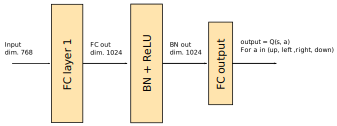
\includegraphics[width=\textwidth]{network}
\end{frame}
\begin{frame}{Training hyper-parameters}
	\begin{itemize}
	\item The network is trained for $500$ episodes;
	\item Each episode, the network is updated $1000$ times;
	\item The samples drawn from the Replay Memory in mini-batches of $32$
	\item The discount factor is fixed at $\alpha=0.85$. 
	\item The exploration rate $\epsilon$ starts at $0.9$, linearly decaying until the quarter-way episode until it reaches value $\epsilon = 0.1$. 
	\item The employed SGD optimizer is Adam, with \textit{learning rate} $\eta = 10^{-4}$ and \textit{weight decay} (L2 regularization) $= 10^{-6}$.
	\\~\\
Before computing the action-value function, the state is processed as follows: it is flattened and normalized to fit in the range $[-1,1]$ with the processing $s_{normalized} = (s - 0.5)*2$. 
	
	\item When using the Double-Q Learning, the network are swapped every 5 episodes.
	\end{itemize}

\end{frame}

\subsection{Experimental results}
\begin{frame}{Evaluating the model}
	After the agent plays 1,000 matches of the game, we evaluate our agent in terms of:
	\begin{itemize}
		\item The number of matches terminated with a \textbf{positive rate};
		\item The number of matches terminated on the arrival square (\textbf{Arrivals rate});
		\item The \textbf{average total reward} and \textbf{average positive reward} of all the matches.
		Additionally, this results are sided by the result reached by an "oracle agent", computed as $d(start, finish) + 1$, where $d(*,*)$ is the \textit{Manhattan} distance between two cells.
	\end{itemize} 	


\begin{table}
\resizebox{\textwidth}{!}{%

	\begin{tabular}{l c c c c c}
		\toprule
		Method & Pos. rate (\%) & Arr. rate (\%) & Avg. final reward & Avg. oracle reward \\ 
		\midrule
		DQL & 96.0 & 99.8 & 18.06 & 24.0 $\pm$ 0.05 \\ 
		Double DQL  & 94.5 & 99.5 & 14.65 & 24.0 $\pm$ 0.05\\ 
		\bottomrule
	\end{tabular}
}
\end{table}
\end{frame}

\begin{frame}{Reward per episode curves}
	\begin{columns}[c] % The "c" option specifies centered vertical alignment while the "t" option is used for top vertical alignment
		
		\column{.5\textwidth} % Left column and width
		\begin{figure}
		\includegraphics[width=\textwidth]{rewards_per_epoch_gdim-16_gamma-0.85_nepisodes-500_explorationstop-0.25_b-32_dql-False}
		\caption{Reward curve of DQL algorithm.}
		\end{figure}
		
		\column{.5\textwidth} % Right column and width
		\begin{figure}
		\includegraphics[width=\textwidth]{rewards_per_epoch_gdim-16_gamma-0.85_nepisodes-500_explorationstop-0.25_b-32_dql-True}
		\caption{Reward curve of DoubleDQL algorithm.}
		\end{figure}	

	\end{columns}
\end{frame}

\begin{frame}{Loss curves} 
		\begin{columns}[c] % The "c" option specifies centered vertical alignment while the "t" option is used for top vertical alignment
		
		\column{.5\textwidth} % Left column and width
		\begin{figure}
	\includegraphics[width=\textwidth]{loss_per_epoch_gdim-16_gamma-0.85_nepisodes-500_explorationstop-0.25_b-32_dql-False}
\caption{Loss of DQL algorithm.}
\label{fig:dqlloss}
		\end{figure}
		
		\column{.5\textwidth} % Right column and width
		\begin{figure}
	\includegraphics[width=\textwidth]{loss_per_epoch_gdim-16_gamma-0.85_nepisodes-500_explorationstop-0.25_b-32_dql-True}
\caption{Loss curve of DoubleDQL algorithm.}
\label{fig:doubledqlloss}
		\end{figure}	
		
	\end{columns}
\end{frame}


\begin{frame}
\frametitle{References}
\footnotesize{
\begin{thebibliography}{99} % Beamer does not support BibTeX so references must be inserted manually as below
\bibitem[Mnih, 2013]{p1} Volodymyr Mnih, Koray Kavukcuoglu, David Silver, Alex Graves and Ioannis Antonoglou, Daan Wierstra and Martin Riedmiller
\newblock Playing Atari with Deep Reinforcement Learning (2013)


\bibitem[Van Hassel, 2015]{p1} Deep Reinforcement Learning with Double Q-learning
\newblock Hado van Hasselt and Arthur Guez and David Silver (2015)
\end{thebibliography}
}
\end{frame}

%------------------------------------------------

\begin{frame}
\Huge{\centerline{Thanks for listening!}}
\end{frame}

%----------------------------------------------------------------------------------------

\end{document} 